\chapter{Casi di studio e valutazioni}
In questa sezione verranno riportati i casi studio e i test effettuati sul framework. Tutti questi casi studio sono stati eseguiti su un sistema HPC Galielo-100 Cineca con le specifiche riportate nella tabella sotto

\vspace{.7cm}
\begin{center}

\begin{tabular}{l|l}
    \hline
    \textbf{Parameter} & \textbf{Value} \\
    \hline
    Number of nodes used & 3 \\
    \hline
    Processor & Intel CascadeLake 8260 \\
    \hline
    Number of sockets per node & 2 \\
    \hline
    Number of cores per socket & 24 \\
    \hline
    Memory size per node & 384 GB \\
    \hline
    Interconnect & Mellanox Infiniband 100GbE \\
    \hline
    OS & CentOS Linux \\ 
    \hline
    MPI & Open MPI  4.1.1 \\
    \hline
\end{tabular}
\label{table:hpc}
\end{center}


\section{Test}
Sono stati svolti diversi test al fine di creare un modello per l'utilizzo e la caratterizzazione di DDS, ed in particolare è stata usato FastDDS, all'interno di sitemi HPC, nel contesto del Power Management. 

In particolare nel Publisher \ref{actor:publisher} prima e dopo la chiamata a funzione di write() %TODO: inserire nella tesi?
si sono presi i valori time-invio, istruzioni, e TSC, mentre al lato ricevente, di Subscriber \ref{actor:subscriber} è stato preso il tempo al momento dell'arrivo del messaggio. In questo modo si sono misurati i seguenti parametri:
\begin{itemize}
    \item Tempo solo invio
    \item Tempo invio-ricezione
    \item Perf-Event Instructions
    \item TSC (read\_tsc)
\end{itemize}
%TODO: se serve approfondire TSC, e metriche eseguite prima e dopo
%TODO: Struttura SUB e PUB con i vari UML
\subsection{Sincronizzazione orologi su nodi diversi}
Per ottenere risultati attendibili sulla metrica del tempo è stato necessario sincronizzare i nodi utilizzati prima di poter far partire i test. Per farlo è stato usata una funzione \emph{CLOCK\_MONOTONIC} che rappresenta un \textit{un orologio non impostabile a livello di sistema che rappresenta il tempo monotono da un punto non specificato nel passato. Su Linux, quel punto corrisponde al numero di secondi di esecuzione del sistema da quando è stato avviato. L'orologio CLOCK\_MONOTONIC non è influenzato da salti discontinui nell'ora del sistema, ma è influenzato dalle regolazioni incrementali eseguite da  NTP.} Il problema che si è presentato, è che avendo nodi diversi su cui far eseguire i test, per provare ad esempio nel modo più affidabile i protocolli di trasporto, è stato necessario implementare delle MPI\_Barrier prima di diverse esecuzioni di \emph{clock\_gettime(CLOCK\_MONOTONIC)}. Di seguito sono stati riportati i grafici del risultato ottenuto.
\begin{figure}[H]
    \centering
    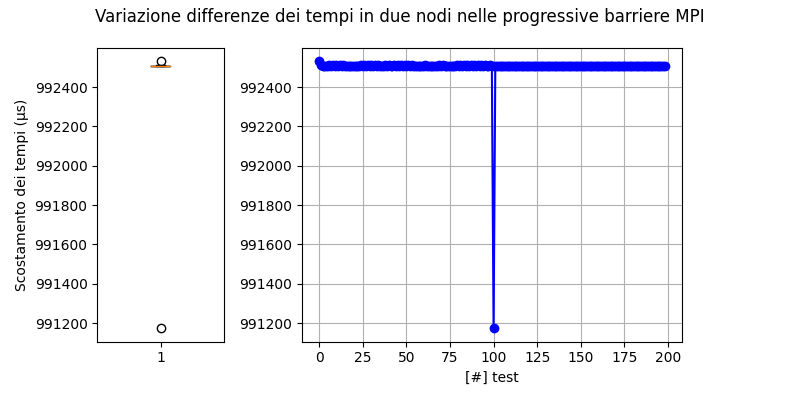
\includegraphics[width=\textwidth]{./results/time_sync_node.png}
    \caption{Scostamento del tempo su nodi diversi}
    \label{fig:sync_time_shift}
    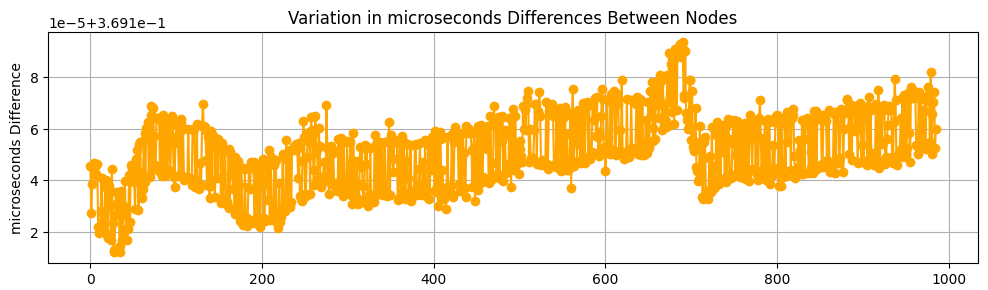
\includegraphics[width=0.99\textwidth]{./results/time_shift_clean.png}
    \caption{Scostamento senza outliers}
    \label{fig:sync_diff_distr}
    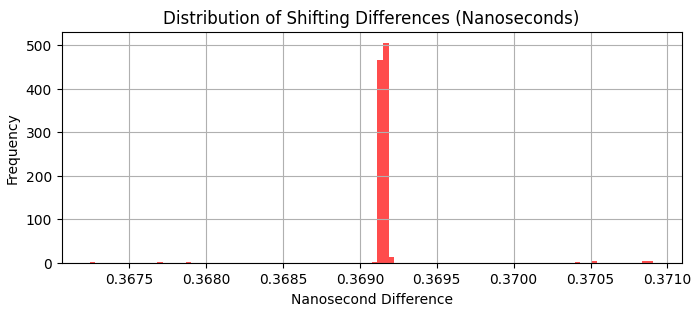
\includegraphics[width=\textwidth]{./results/time_sync_distribution.png}
    \caption{Distribuzione delle differenze}
    \label{fig:sync_diff_distr}
\end{figure}

Come possibile vedere nella figura \ref{fig:sync_time_shift} nonostante le mpi\_barrier, sono presenti degli scostamenti di tempo tra 2 nodi durante diversi test effettuati (in particolare 1000), e si è scelto di utilizzare il valore modale di questa differenza,sulla base del quale, si sono elaborati tutti i dati successivi.

\subsection{Impatto del numero di sub in un dominio}
Visto lo schema %TODO: UML
risulta facile capire, che il numero di subscriber presenti in un dominio comporta un overhead di comunicazione che va ad influenzare sia i tempi, che i cicli impiegati nella singola \emph{publish} su un topic
\begin{figure}[H]
    \centering
    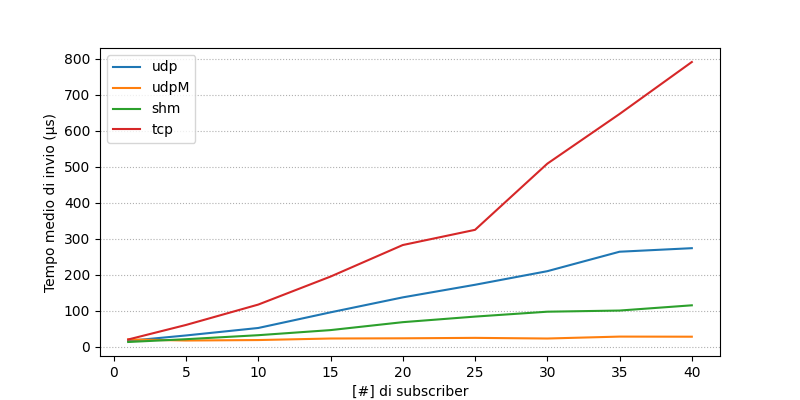
\includegraphics[width=\textwidth]{./results/test3_sending_multiplesub.png} %TODO, sqeunce is an error
    \caption{overhead sulla publish all'aumentare dei subscriber}
    \label{fig:test3_overhead}
\end{figure}
che viene facilmente dimostrato nella figura\ref{fig:test3_overhead}. Ovviamente l'impatto è poco significativo in quei protocolli che applicano strutture di multicasting %TODO: aggiungere nel glossario
come udp-Multicast e Shared-Memory. Questo può portare una singola publish a impiegare più cicli e più tempo della singola ricezione dei messaggi, come si vede nella figura\ref{fig:test3_different_protocols}
\begin{figure}[H]
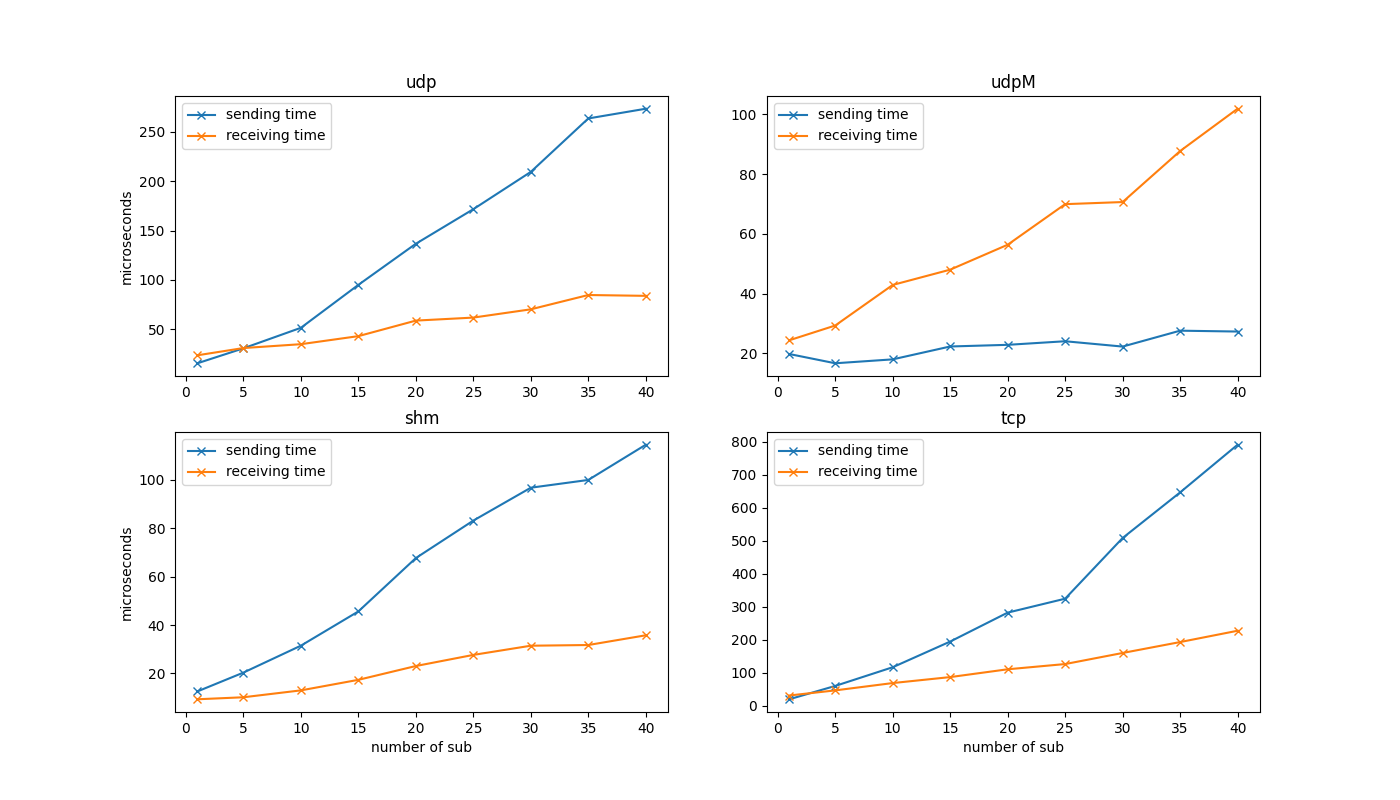
\includegraphics[width=\textwidth]{./results/test3_different_protocol_send_receive.png} %TODO, sqeunce is an error
    \caption{differenza tra solo publish e publish-subscribe per ogni protocollo}
    \label{fig:test3_different_protocols}
\end{figure}
In tutti i test successivi, ove non specificato diversamente sono stati usati 1 publisher e 48 subscriber su diversi nodi. Questo è stato fatto per provare la scalabilità, visto che nel testbed che è stato utilizzato, erano presenti 48 core (1 core per ogni subscriber).

\subsection{Test1}
Nel primo test si è valutata la differenza di diversi protocolli di trasporto utilizzando la rete infiniband \ref{table:hpc} su diversi nodi di un supercalcolatore. In particolare si è voluta sottolineare la differenza di tempi e cicli usando i diversi protocolli di comunicazione offerti da RTPS:
\begin{itemize}
    \item udp
    \item tcp 
    \item udp-multicast % TODO: uml
    \item shared-memory
\end{itemize}

io risultati che sono stati trovati forniscono importanti informazioni,
\begin{figure}[H]
    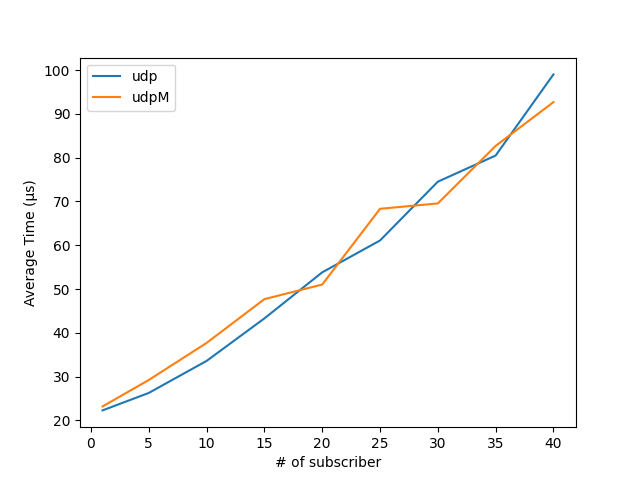
\includegraphics[width=\textwidth]{./results/test3_udpvsudpM.png} %TODO, sqeunce is an error
        \caption{}
        \label{}
\end{figure}

%NPUB NSub
\subsection{Test2}
\subsection{Test3}

\section{Risultati}
\section{Modello}
\section{Scheletro componenti}
Nel seguente capitolo viene stilato uno scheletro dei componenti con i relativi topic usati al fine di dare una visione completa e aggiuntiva rispetto al modello precedentemente stilato  
\begin{figure}[H]
    \centering
    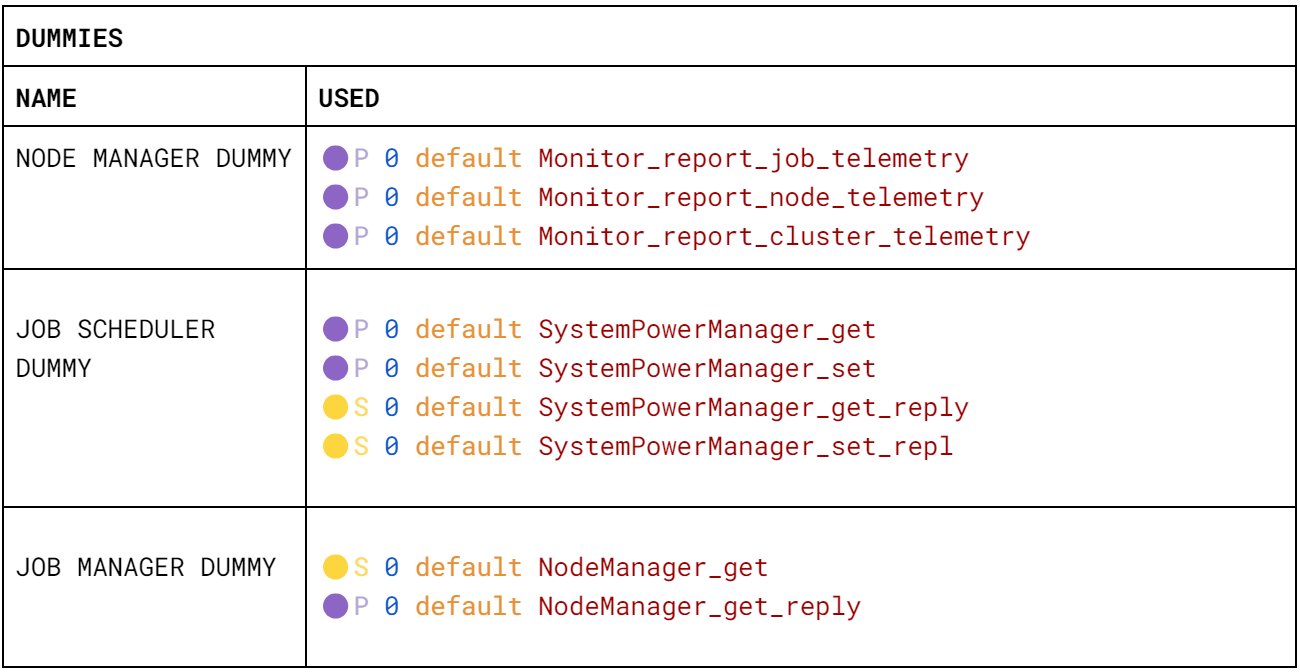
\includegraphics[width=\textwidth]{./img/dummies_skeleton.png}
    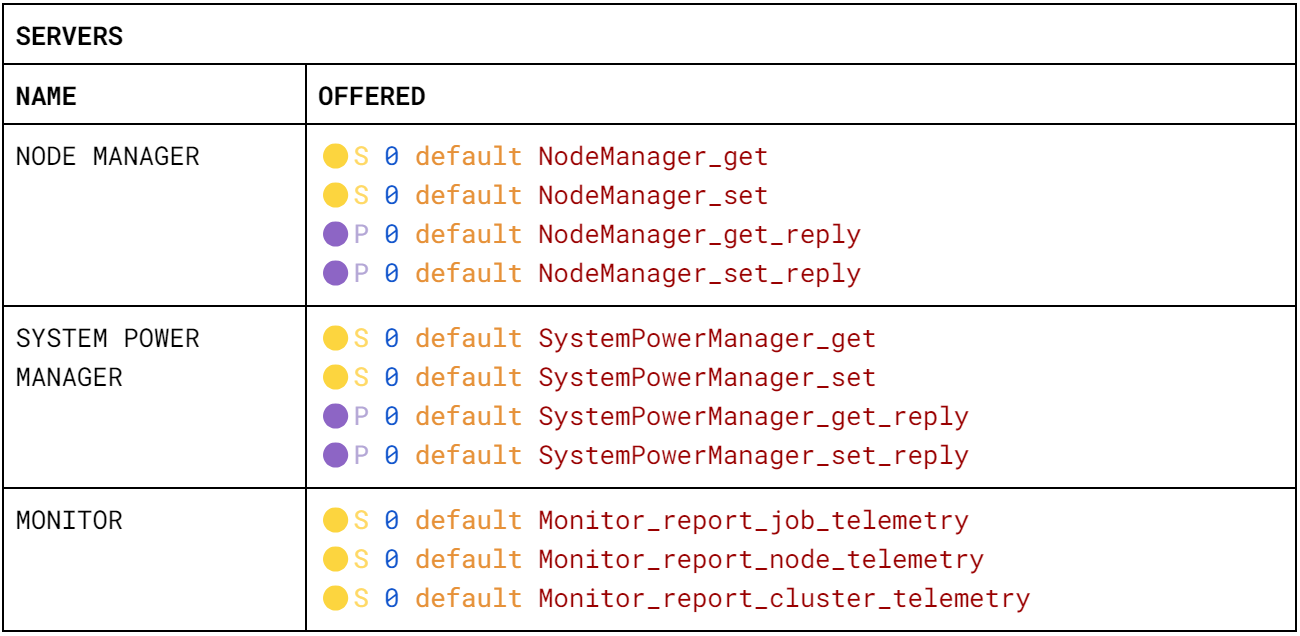
\includegraphics[width=\textwidth]{./img/server_skeleton.png}
\end{figure}
